\documentclass[tikz,border=4pt]{standalone}
\begin{document}
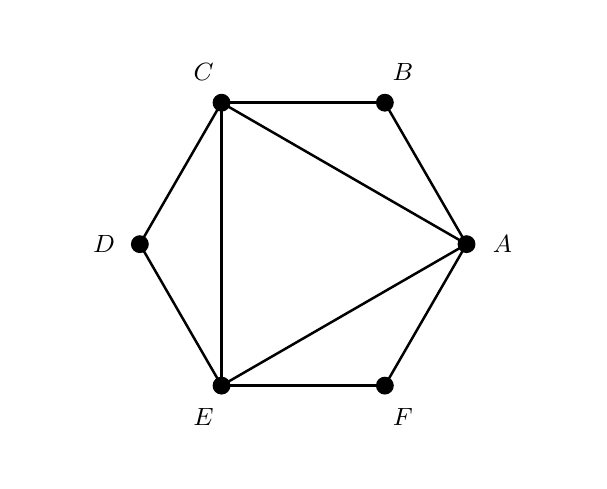
\begin{tikzpicture}[x=0.025cm,y=-0.025cm]
\path[use as bounding box] (0,0) rectangle (280,220);
\path[draw=black,fill=none,line width=0.8999999999999999pt,line join=round] (223,110) -- (181.5,38.1199);
\path[draw=black,fill=none,line width=0.8999999999999999pt,line join=round] (181.5,38.1199) -- (98.5,38.1199);
\path[draw=black,fill=none,line width=0.8999999999999999pt,line join=round] (98.5,38.1199) -- (57,110);
\path[draw=black,fill=none,line width=0.8999999999999999pt,line join=round] (57,110) -- (98.5,181.8801);
\path[draw=black,fill=none,line width=0.8999999999999999pt,line join=round] (98.5,181.8801) -- (181.5,181.8801);
\path[draw=black,fill=none,line width=0.8999999999999999pt,line join=round] (181.5,181.8801) -- (223,110);
\path[draw=black,fill=none,line width=0.8999999999999999pt,line join=round] (223,110) -- (98.5,38.1199);
\path[draw=black,fill=none,line width=0.8999999999999999pt,line join=round] (98.5,38.1199) -- (98.5,181.8801);
\path[draw=black,fill=none,line width=0.8999999999999999pt,line join=round] (98.5,181.8801) -- (223,110);
\path[draw=black,fill=black,line width=.75pt] (223,110) circle[radius=0.1cm];
\node[font=\small,inner sep=0pt] at (241.26,110) {$A$};
\path[draw=black,fill=black,line width=.75pt] (181.5,38.1199) circle[radius=0.1cm];
\node[font=\small,inner sep=0pt] at (190.63,22.3063) {$B$};
\path[draw=black,fill=black,line width=.75pt] (98.5,38.1199) circle[radius=0.1cm];
\node[font=\small,inner sep=0pt] at (89.37,22.3063) {$C$};
\path[draw=black,fill=black,line width=.75pt] (57,110) circle[radius=0.1cm];
\node[font=\small,inner sep=0pt] at (38.74,110) {$D$};
\path[draw=black,fill=black,line width=.75pt] (98.5,181.8801) circle[radius=0.1cm];
\node[font=\small,inner sep=0pt] at (89.37,197.6937) {$E$};
\path[draw=black,fill=black,line width=.75pt] (181.5,181.8801) circle[radius=0.1cm];
\node[font=\small,inner sep=0pt] at (190.63,197.6937) {$F$};
\end{tikzpicture}
\end{document}
